\documentclass[12pt]{article}
\usepackage[a4paper, margin=0.75in]{geometry}
\usepackage{graphicx}
\usepackage{amsmath}
\usepackage{float}
\usepackage[colorlinks=false, pdfborder={0 0 0}]{hyperref}
\usepackage{caption}

\title{\textbf{GridWorld - Q-Learning Report}}
\author{Satish Jhanwer (G24AIT009)}
\date{\today}

\begin{document}

\maketitle
\tableofcontents
\newpage
\listoffigures
\newpage

\section{Part 1: Epsilon-Greedy Q-Learning}

\subsection{Environment Setup}
\begin{itemize}
  \item Grid size: 5x5
  \item Start: (1, 1)
  \item Goal: (5, 5), Reward = \(+5\)
  \item Trap: (3, 5), Reward = \(-5\)
  \item Obstacles: (1,4), (2,2), (3,3), (5,3)
  \item Stepping outside the grid yields a reward of \(-1\); all other moves yield 0.
  \item Learning rate (alpha): \(0.1\)
  \item Episodes: 100,000
\end{itemize}

\subsection{Converged Policy and Value Function}
I applied epsilon-greedy Q-learning with: Gamma = \(0.9\) and Epsilon = \(0.2\)

\begin{figure}[htbp]
  \centering
  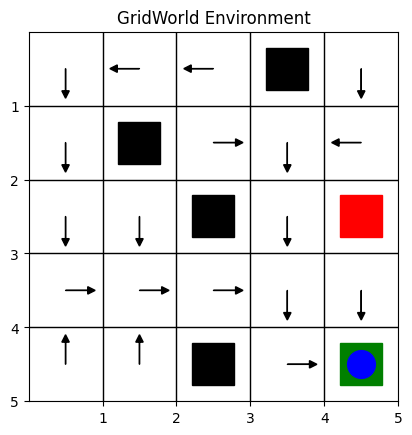
\includegraphics[width=0.48\textwidth]{images/part1_q1_policy.png}
  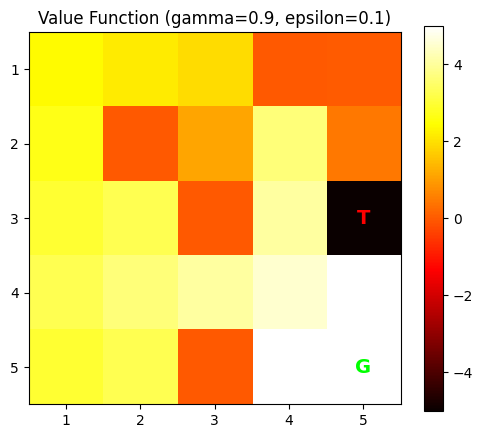
\includegraphics[width=0.48\textwidth]{images/part1_q1_value.png}
  \caption{Policy and Value Function}
\end{figure}

\textbf{Interpretation:}
\begin{itemize}
  \item The agent learned an optimal policy, efficiently navigating around obstacles and avoiding the trap.
  \item High values propagate from the goal, while states near the trap show significantly lower values, reflecting effective risk awareness.
  \item The results demonstrate efficient convergence through epsilon-greedy updates.
\end{itemize}

\newpage
\subsection{Varying Discount Factor (Gamma) - Fixed Epsilon = 0.1}
Gamma values tested: \(0.1, 0.5, 0.9\)

\begin{figure}[htbp]
  \centering
  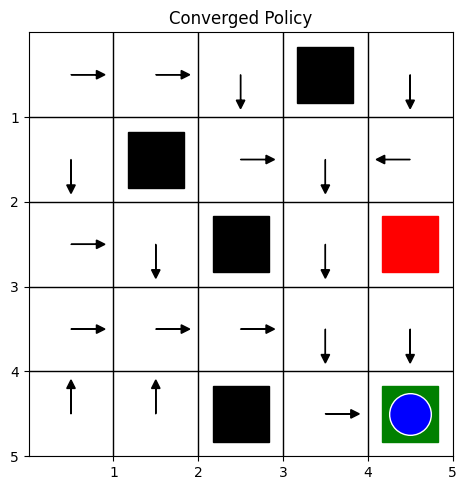
\includegraphics[width=0.48\textwidth]{images/part1_q2_gamma_0.1_policy.png}
  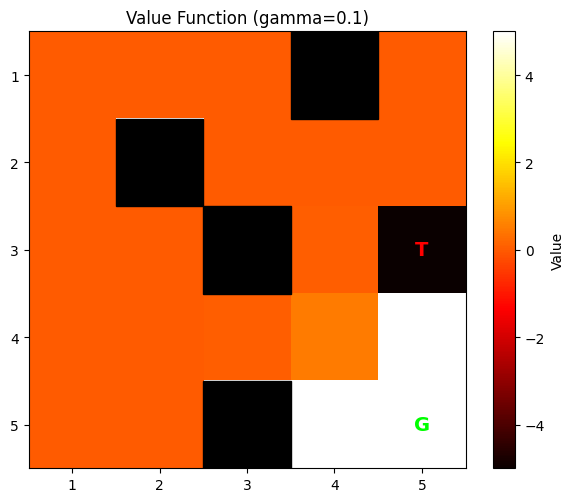
\includegraphics[width=0.48\textwidth]{images/part1_q2_gamma_0.1_value.png}
  \caption{Gamma = 0.1: Policy and Value Function}
\end{figure}

\begin{figure}[htbp]
  \centering
  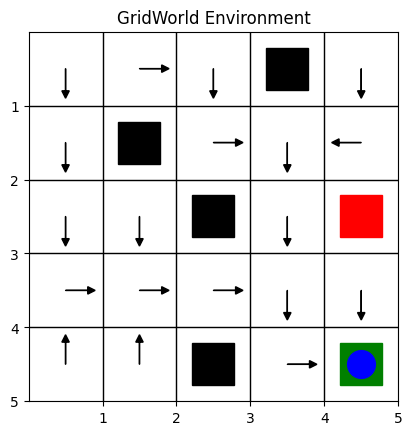
\includegraphics[width=0.48\textwidth]{images/part1_q2_gamma_0.5_policy.png}
  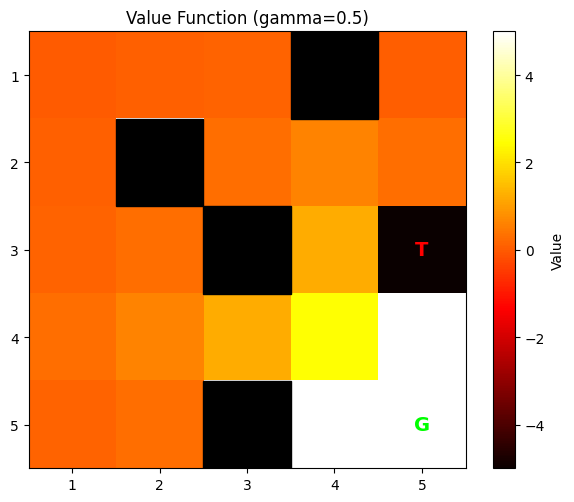
\includegraphics[width=0.48\textwidth]{images/part1_q2_gamma_0.5_value.png}
  \caption{Gamma = 0.5: Policy and Value Function}
\end{figure}

\begin{figure}[htbp]
  \centering
  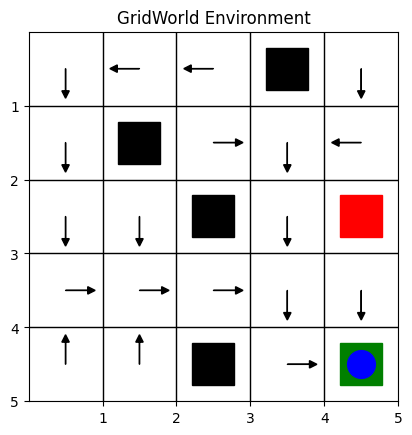
\includegraphics[width=0.48\textwidth]{images/part1_q2_gamma_0.9_policy.png}
  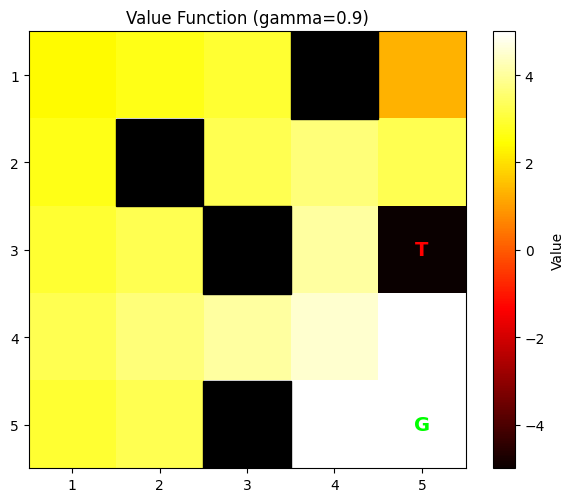
\includegraphics[width=0.48\textwidth]{images/part1_q2_gamma_0.9_value.png}
  \caption{Gamma = 0.9: Policy and Value Function}
\end{figure}

\begin{figure}[H]
  \centering
  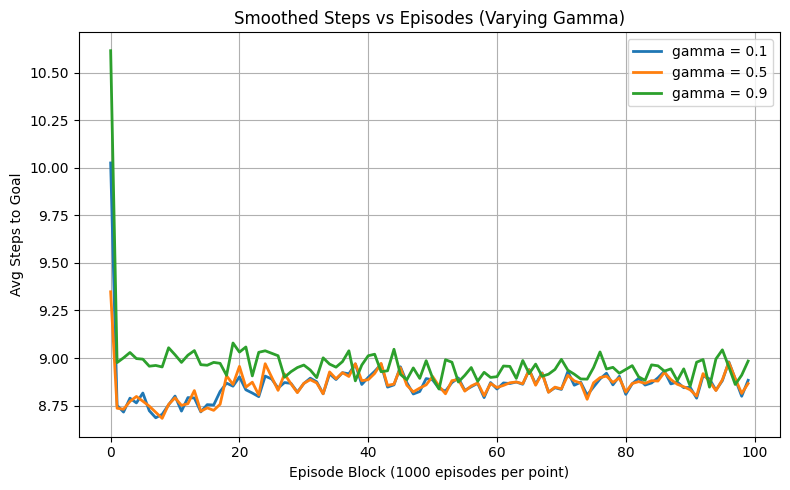
\includegraphics[width=0.85\textwidth]{images/part1_q2_steps_vs_gamma.png}
  \caption{Steps to Goal for Different Gamma Values}
\end{figure}

\textbf{Interpretation:}
\begin{itemize}
  \item Gamma = 0.1, the agent strongly prefers immediate rewards and often ignores the goal's distant reward, resulting in \mbox{short-sighted} and suboptimal paths.
  \item Gamma = 0.5, encourages the agent to recognize longer-term rewards, but it still occasionally diverges.
  \item Gamma = 0.9, promotes long-term planning, enabling the agent to follow the most optimal and direct paths to the goal.
  \item Gamma = 0.9, The step plot confirms that higher gamma values lead to smoother convergence due to better foresight.
\end{itemize}

\subsection{Varying Epsilon - Fixed Gamma = 0.9}
Epsilon values tested: \(0.1, 0.3, 0.5\)

\begin{figure}[htbp]
  \centering
  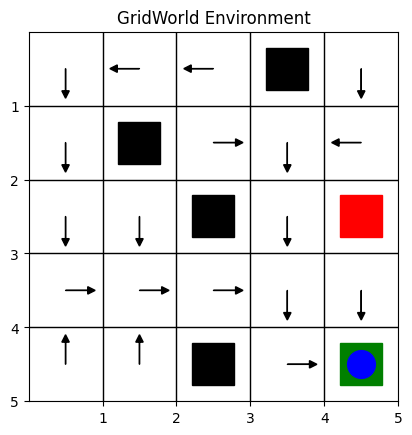
\includegraphics[width=0.48\textwidth]{images/part1_q3_epsilon_0.1_policy.png}
  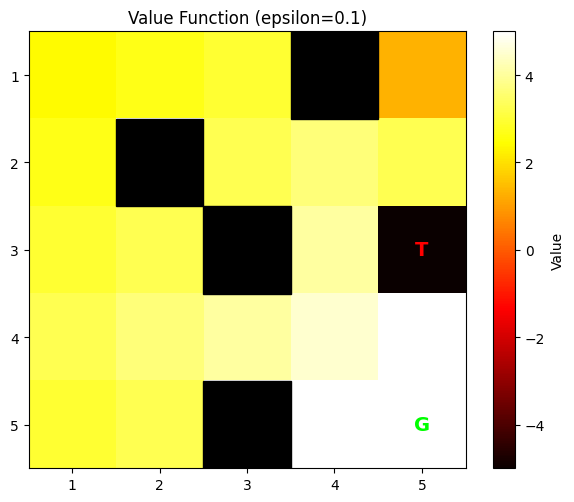
\includegraphics[width=0.48\textwidth]{images/part1_q3_epsilon_0.1_value.png}
  \caption{Epsilon = 0.1: Policy and Value Function}
\end{figure}

\begin{figure}[htbp]
  \centering
  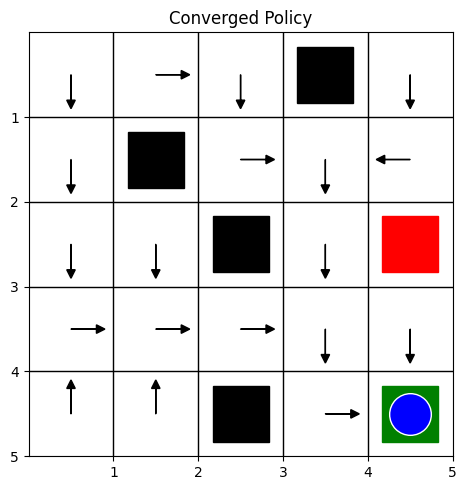
\includegraphics[width=0.48\textwidth]{images/part1_q3_epsilon_0.3_policy.png}
  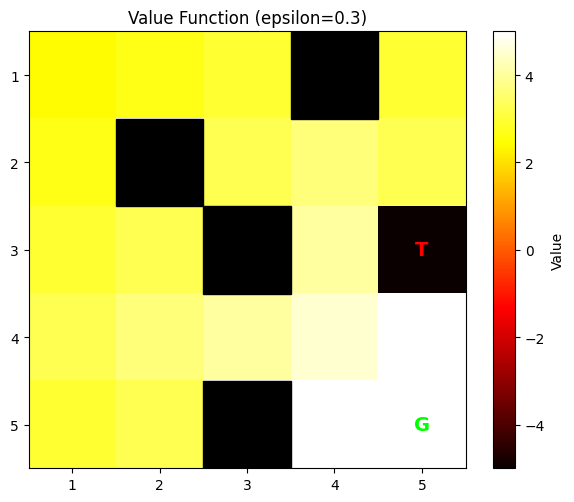
\includegraphics[width=0.48\textwidth]{images/part1_q3_epsilon_0.3_value.png}
  \caption{Epsilon = 0.3: Policy and Value Function}
\end{figure}

\begin{figure}[htbp]
  \centering
  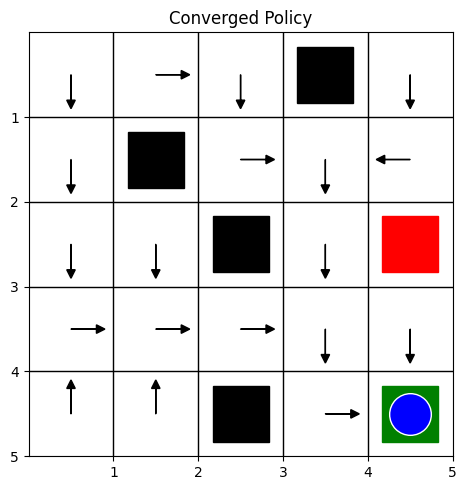
\includegraphics[width=0.48\textwidth]{images/part1_q3_epsilon_0.5_policy.png}
  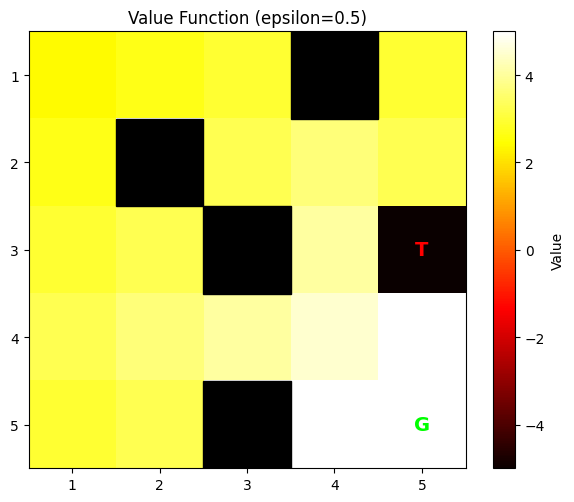
\includegraphics[width=0.48\textwidth]{images/part1_q3_epsilon_0.5_value.png}
  \caption{Epsilon = 0.5: Policy and Value Function}
\end{figure}

\begin{figure}[H]
  \centering
  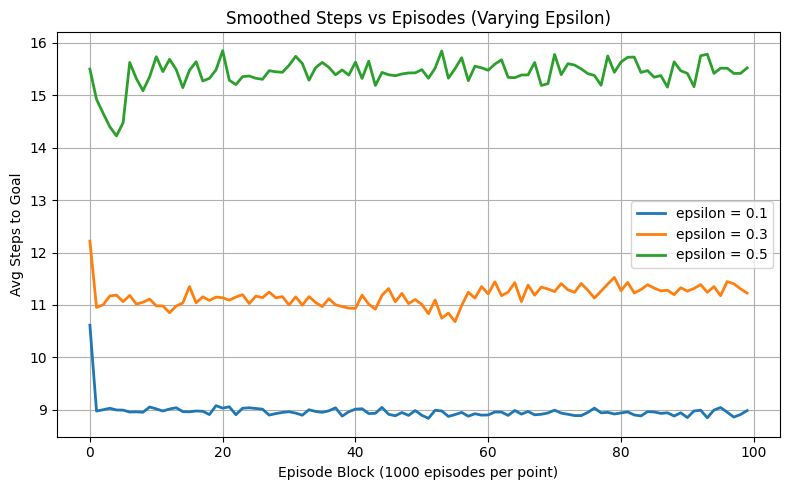
\includegraphics[width=0.85\textwidth]{images/part1_q3_steps_vs_epsilon.png}
  \caption{Steps to Goal for Different Epsilon Values}
\end{figure}

\textbf{Interpretation:}
\begin{itemize}
  \item Epsilon= 0.1 encourages greedy exploitation, resulting in fast convergence but possibly missing better paths early in learning.
  \item Epsilon= 0.3 introduces moderate exploration, allowing the agent to explore alternatives but causing slower convergence.
  \item Epsilon = 0.5 increases randomness, which leads to inefficient learning and significantly delayed convergence.
  \item Lower epsilon values promote stability and help the agent discover the optimal path more quickly, as reflected in fewer average steps per episode.
\end{itemize}

\section{Part 2: Softmax-Based Q-Learning}

\subsection{Environment Setup}
\begin{itemize}
  \item Grid size: 5x11
  \item Start: (1, 1)
  \item Goal: (5, 11), Reward = \(+5\)
  \item Trap: (4, 7), Reward = \(-5\)
  \item Tunnels: ((3, 5), (3, 6))
  \item Obstacles: (2,3), (3,3), (4,3), (3,9), (3,10), (5,9)
  \item Stepping outside the grid yields a reward of \(-1\); all other moves yield 0.
  \item Learning rate (alpha): \(0.1\)
  \item Episodes: 200,000
\end{itemize}

\subsection{Converged Policy and Value Function (Softmax)}
\begin{itemize}
  \item Gamma = \(0.9\)
  \item Tau (softmax temperature) = \(0.1\)
\end{itemize}

\begin{figure}[H]
  \centering
  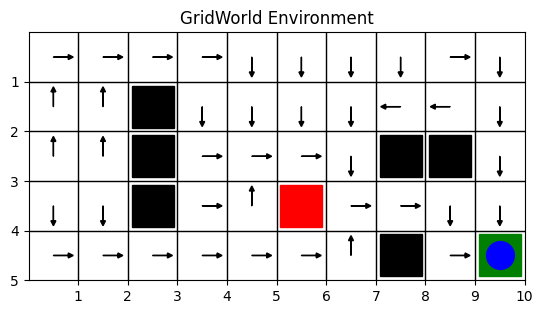
\includegraphics[width=0.85\textwidth]{images/part2_q1_policy.png}
  \caption{Converged Policy (Softmax)}
\end{figure}
\begin{figure}[H]
  \centering
  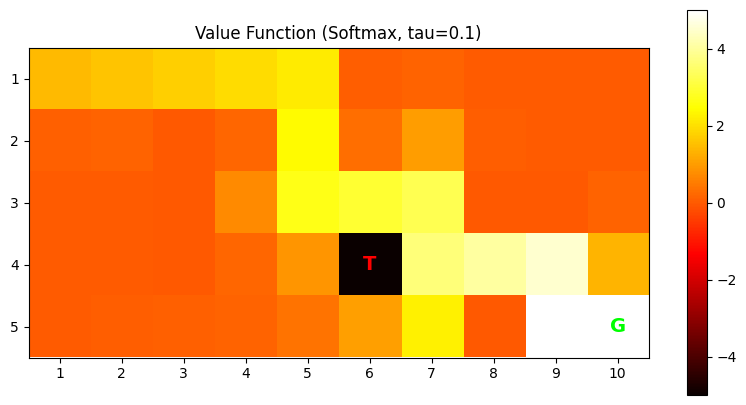
\includegraphics[width=0.85\textwidth]{images/part2_q1_value.png}
  \caption{Value Function (Softmax)}
\end{figure}

\textbf{Interpretation:}
\begin{itemize}
  \item Softmax exploration introduces early stochasticity but enables the agent to eventually converge to the optimal path.
  \item Despite the increased grid complexity, the agent effectively navigates through the bottleneck, avoiding traps and dead-ends.
  \item The value gradient clearly reflects proximity to the goal.
\end{itemize}

\newpage
\subsection{Varying Gamma - Fixed Tau = 0.1}
Gamma values tested: \(0.1, 0.5, 0.9\)

\begin{figure}[H]
  \centering
  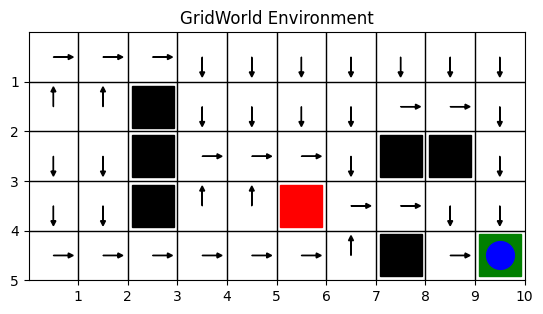
\includegraphics[width=0.85\textwidth]{images/part2_q2_gamma_0.1_policy.png}
  \caption{Gamma = 0.1 Policy}
\end{figure}
\begin{figure}[H]
  \centering
  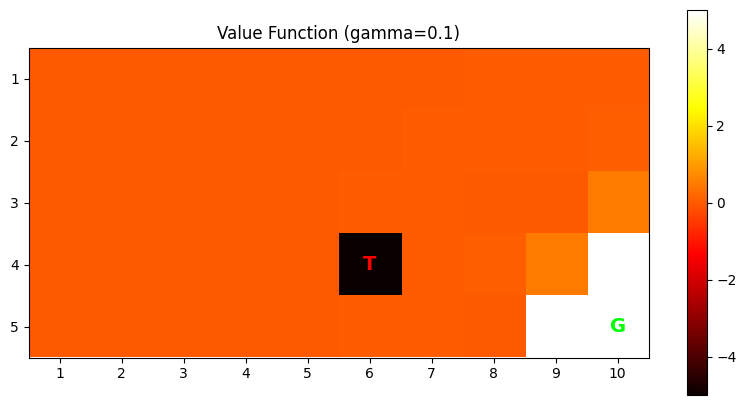
\includegraphics[width=0.85\textwidth]{images/part2_q2_gamma_0.1_value.png}
  \caption{Gamma = 0.1 Value Function}
\end{figure}

\begin{figure}[H]
  \centering
  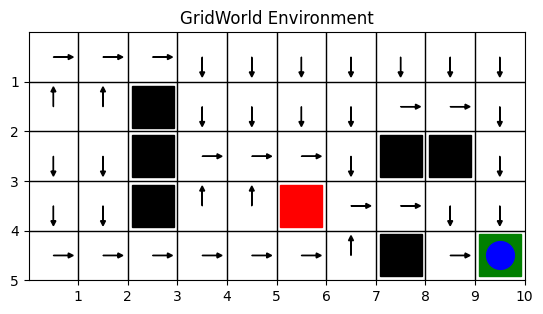
\includegraphics[width=0.85\textwidth]{images/part2_q2_gamma_0.5_policy.png}
  \caption{Gamma = 0.5 Policy}
\end{figure}
\begin{figure}[H]
  \centering
  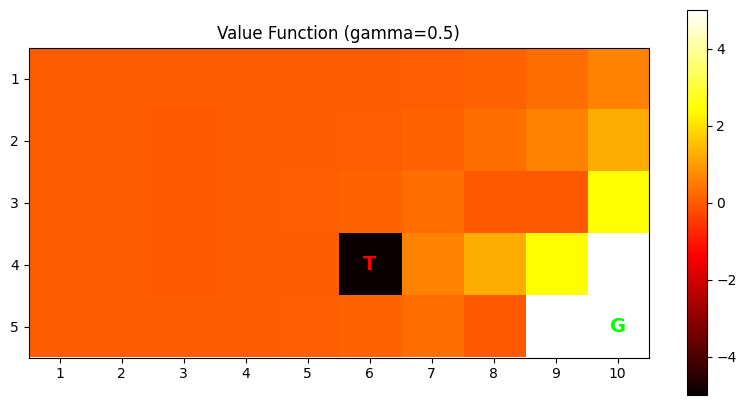
\includegraphics[width=0.85\textwidth]{images/part2_q2_gamma_0.5_value.png}
  \caption{Gamma = 0.5 Value Function}
\end{figure}

\begin{figure}[H]
  \centering
  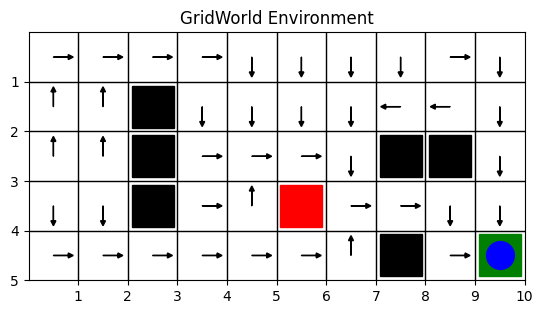
\includegraphics[width=0.85\textwidth]{images/part2_q2_gamma_0.9_policy.png}
  \caption{Gamma = 0.9 Policy}
\end{figure}
\begin{figure}[H]
  \centering
  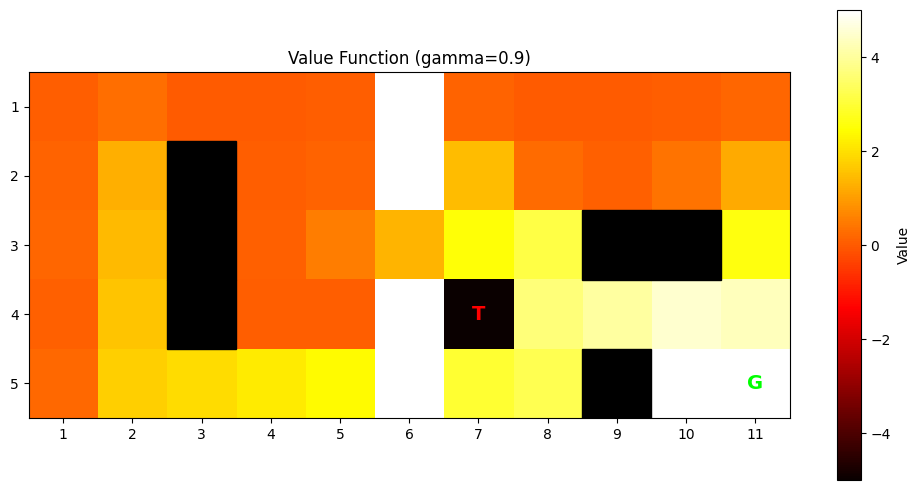
\includegraphics[width=0.85\textwidth]{images/part2_q2_gamma_0.9_value.png}
  \caption{Gamma = 0.9 Value Function}
\end{figure}

\begin{figure}[H]
  \centering
  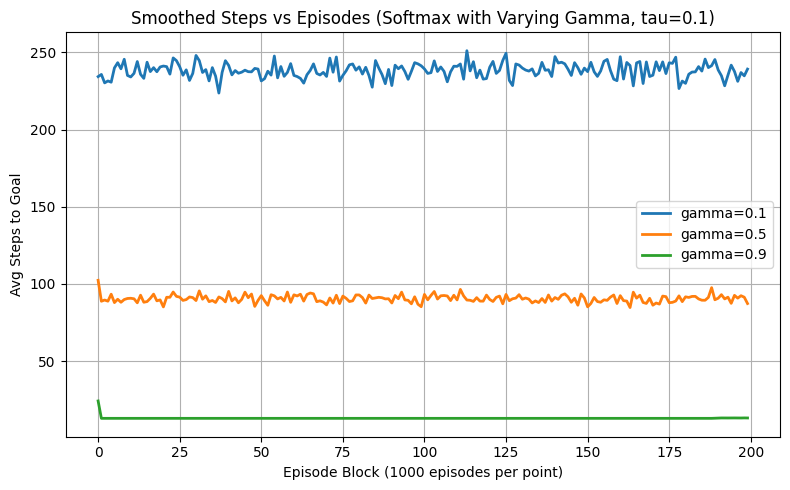
\includegraphics[width=0.85\textwidth]{images/part2_q2_steps_vs_gamma.png}
  \caption{Steps to Goal for Different Gamma Values}
\end{figure}

\textbf{Interpretation:}
\begin{itemize}
  \item With Gamma = 0.1 the agent behaves short-sightly and struggles with the bottleneck corridor.
  \item Gamma = 0.5 improves navigation, but some indecisiveness remains.
  \item Gamma = 0.9 enables the agent to learn an optimal long-horizon policy and consistently avoid traps.
  \item The plot shows a steady reduction in average steps as gamma increases.
\end{itemize}

\newpage
\subsection{Varying Tau - Fixed Gamma = 0.9}
Tau values tested: \(0.1, 0.3, 0.5\)

\begin{figure}[H]
  \centering
  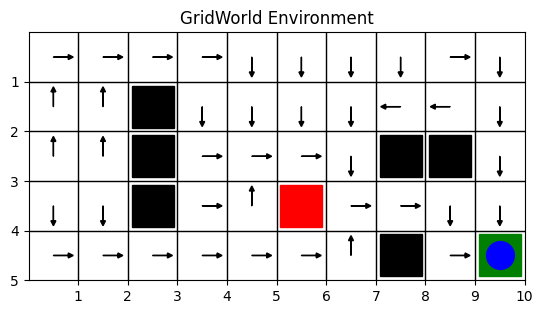
\includegraphics[width=0.85\textwidth]{images/part2_q3_tau_0.1_policy.png}
  \caption{Tau = 0.1 Policy}
\end{figure}
\begin{figure}[H]
  \centering
  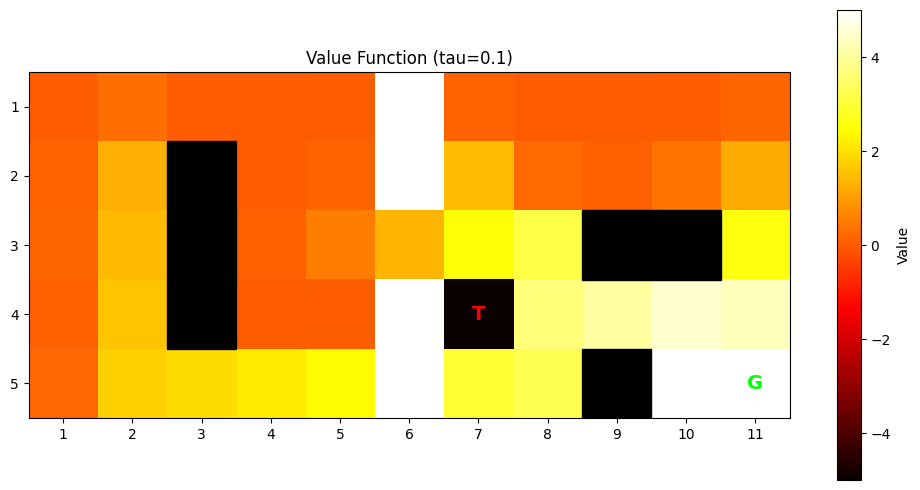
\includegraphics[width=0.85\textwidth]{images/part2_q3_tau_0.1_value.png}
  \caption{Tau = 0.1 Value Function}
\end{figure}

\begin{figure}[H]
  \centering
  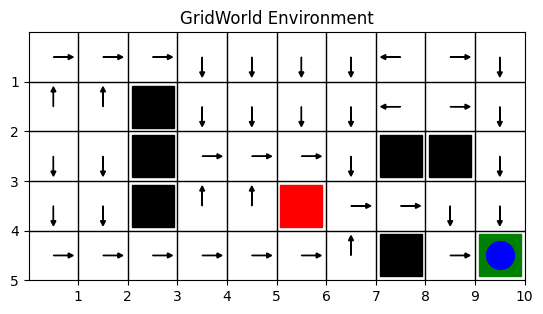
\includegraphics[width=0.85\textwidth]{images/part2_q3_tau_0.3_policy.png}
  \caption{Tau = 0.3 Policy}
\end{figure}
\begin{figure}[H]
  \centering
  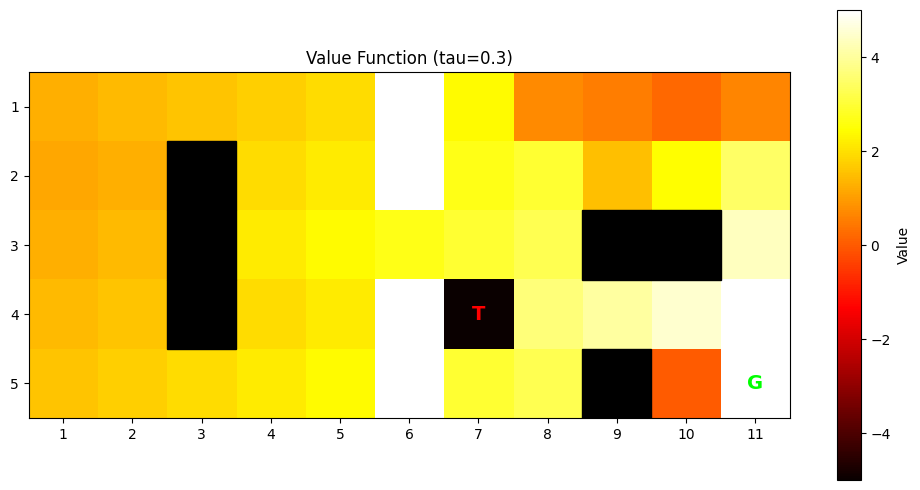
\includegraphics[width=0.85\textwidth]{images/part2_q3_tau_0.3_value.png}
  \caption{Tau = 0.3 Value Function}
\end{figure}

\begin{figure}[H]
  \centering
  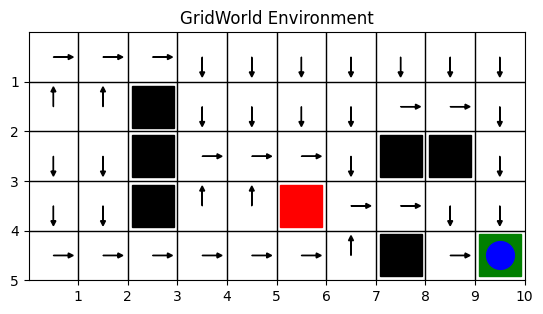
\includegraphics[width=0.85\textwidth]{images/part2_q3_tau_0.5_policy.png}
  \caption{Tau = 0.5 Policy}
\end{figure}
\begin{figure}[H]
  \centering
  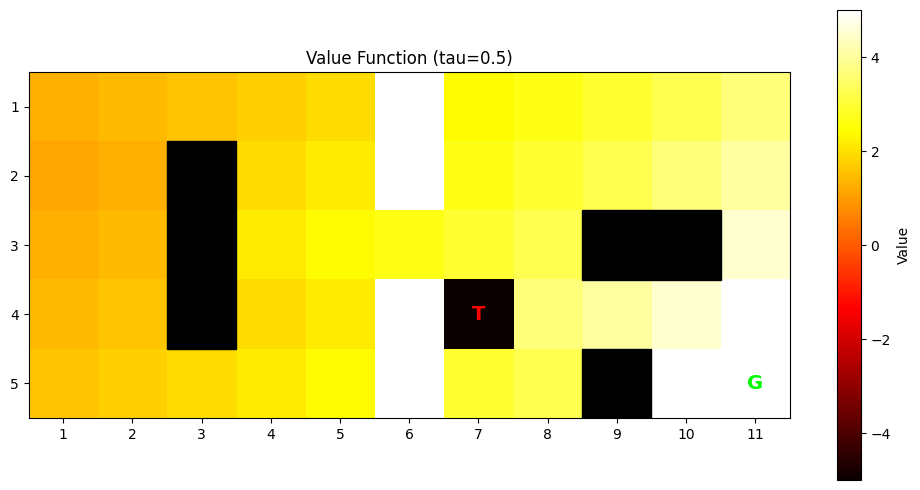
\includegraphics[width=0.85\textwidth]{images/part2_q3_tau_0.5_value.png}
  \caption{Tau = 0.5 Value Function}
\end{figure}

\begin{figure}[H]
  \centering
  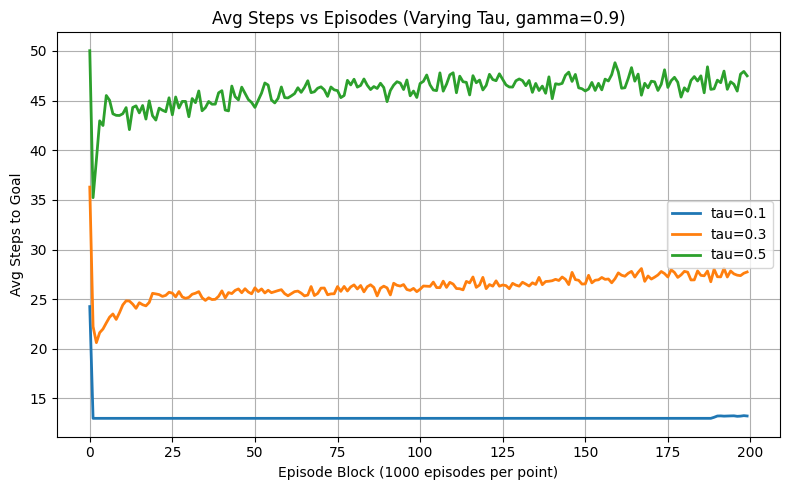
\includegraphics[width=0.85\textwidth]{images/part2_q3_steps_vs_tau.png}
  \caption{Steps to Goal for Different Tau Values}
\end{figure}

\textbf{Interpretation:}
\begin{itemize}
  \item Tau = 0.1 produces near-deterministic softmax decisions, allowing efficient convergence and high policy quality.
  \item Tau = 0.3 balances exploration and exploitation, resulting in moderate performance.
  \item Tau = 0.5 makes the policy overly exploratory, flattening action selection probabilities and degrading performance.
  \item Increasing tau causes the agent to act too randomly, which hampers learning stability.
\end{itemize}

\section{Conclusion}
\begin{itemize}
  \item Both epsilon-greedy and softmax Q-learning methods perform effectively under suitable configurations.
  \item Low epsilon or tau values accelerate convergence but may cause premature exploitation.
  \item High gamma values consistently improve value propagation and path optimality.
  \item The grid's complexity and layout influence the ideal parameter settings.
\end{itemize}

\section{Appendix}
\begin{itemize}
  \item I structured all code to be modular and reusable.
  \item I ran experiments using Python 3.12.3, NumPy, and Matplotlib (visualizations).
  \item I performed all experiments on a personal workstation (no GPU).
  \item I smoothed graphs using 1000-episode windows for clearer trends.
  \item All scripts are parameterized for easy testing with different grid setups.
\end{itemize}

\end{document}
